\documentclass[a4paper, 10pt, conference]{ieeeconf}

\usepackage[dvipsnames]{xcolor}

\usepackage{times}
\usepackage{graphicx}
\usepackage{amssymb}
\usepackage{amsmath}
\usepackage{breakurl}
\def\UrlBreaks{\do\/\do-}
\usepackage{url,hyperref}
\usepackage{algorithm}
\usepackage{algorithmic}
\usepackage[labelfont={bf},font=small]{caption}
\usepackage[none]{hyphenat}
\usepackage{mathtools, cuted}
\usepackage[noadjust, nobreak]{cite}
\usepackage{tabularx}
\newcolumntype{Y}{>{\centering\arraybackslash}X}
\usepackage{afterpage}
\usepackage{stfloats}
\usepackage{comment}
\usepackage{xcolor,colortbl}

\newcommand{\specialcell}[2][c]{%
  \begin{tabular}[#1]{@{}c@{}}#2\end{tabular}}

\title{\LARGE \bf
Rubin Observatory Science Pipelines on AWS
}

\author{
    Dino Bektesevic$^1$, Andrew Connolly$^1$ \\
    Department of Astronomy, University of Washington \\ Email: dinob@uw.edu, ajc@uw.edu
    }

\begin{document}


\maketitle


%%%%%%%%%%%%%%%%%%%%%%%%%%%%%%%%%%%%%%%%%%%%%%%%%%%%%%%%%%%%%%%%%%%%%%%%%%%%%%%%
\begin{abstract}

The Legacy Survey of Space and Time\footnote{\url{www.lsst.org}} (LSST) aims to conduct a longitudinal 10 year long survey in which the entire night sky will be imaged every three nights. It is estimated LSST will produce 20TB of raw data per night and that, in the 10 years of operations it will deliver a total of 500 petabytes (PB) of data. In this paper we claim that the, pervasive in field of astronomy, subset-download-process paradigm of data reprocessing faces significant challenges at LSST data volumes. We describe an gateway for astronomical science that would allow astronomers to work images and catalogs at scale. As a first step towards that goal we focus on executing LSST's Science Pipelines, a collection of image and catalog processing algorithms, on Amazon Web Services (AWS). We describe Pegasus Workflow Management System\footnote{\url{https://pegasus.isi.edu}} and HTCondor\footnote{\url{https://research.cs.wisc.edu/htcondor/}} can be used to describe, plan and execute a data processing pipelines and manage compute resources. We discuss performance, scalability and cost of deploying on AWS.
\end{abstract}

%%%%%%%%%%%%%%%%%%%%%%%%%%%%%%%%%%%%%%%%%%%%%%%%%%%%%%%%%%%%%%%%%%%%%%%%%%%%%%%%
\section{INTRODUCTION}

Currently pervasive model of sub-selecting, transferring to local compute resources and then reprocessing data was successful in context of past sky-surveys such as such as Sloan Digital Sky Survey\cite{York2000} (SDSS) because technological developments and pricing made acquiring sufficient local compute resource affordable. The new generation sky surveys, such as LSST, promise to deliver an order of magnitude more data rendering the subset-download-process paradigm unviable in the long-term. 

Drawing on lessons learned from previous surveys and in order to facilitate scientific discovery LSST reduces the raw data into multiple different, smaller in volume, science products. LSST also offers 10\% of their compute resources for use to in-collaboration scientists. Even though this approach mitigates a lot of associated problems it does not do away with the need to process pixel level data. At LSST's data volumes however, considering even a relatively small subset of data will amount to a large dataset. For example, over the lifetime of the survey a 1\% random subset of the total data still constitutes a 5 PB large dataset - three the size of PanSTARRS, the largest to-date astronomical image dataset. To reprocess even such small subsets of total data, significant computing resources, and subsequently significant initial investments, are required.

We want to provide astronomers with an interface and tools that allow them to process entire LSST nights in hours and to do so at reasonable prices. As a first step towards such a gateway we focus on image data reduction pipelines. Such pipelines usually consist of multiple different sequential steps that remove instrument signature from the data, detect all sources, potentially cross reference them to previously known sources and measure their properties. Additionally coaddition, the stacking of multiple images covering the same area of the sky in order to improve noise properties, and image differencing, in order to remove non-variable sources, are often desired image operations as well. A typical input and output of such a pipeline is shown on figure-\ref{fig:raw2calexp}. There are many different software solutions that perform these tasks but rarely can they be applied at scale or perform all of the described processing steps. Many of existing data reduction pipelines are conglomerations of bespoke written code and such pre-existing solutions, leaving the astronomical image data reduction landscape in a fragmented state where usually only the larger observatories and sky surveys offer tools to scientists that allow for complete data reduction to take place, and often these tools are difficult to set-up and use. 

\begin{figure}[htb]
\centering
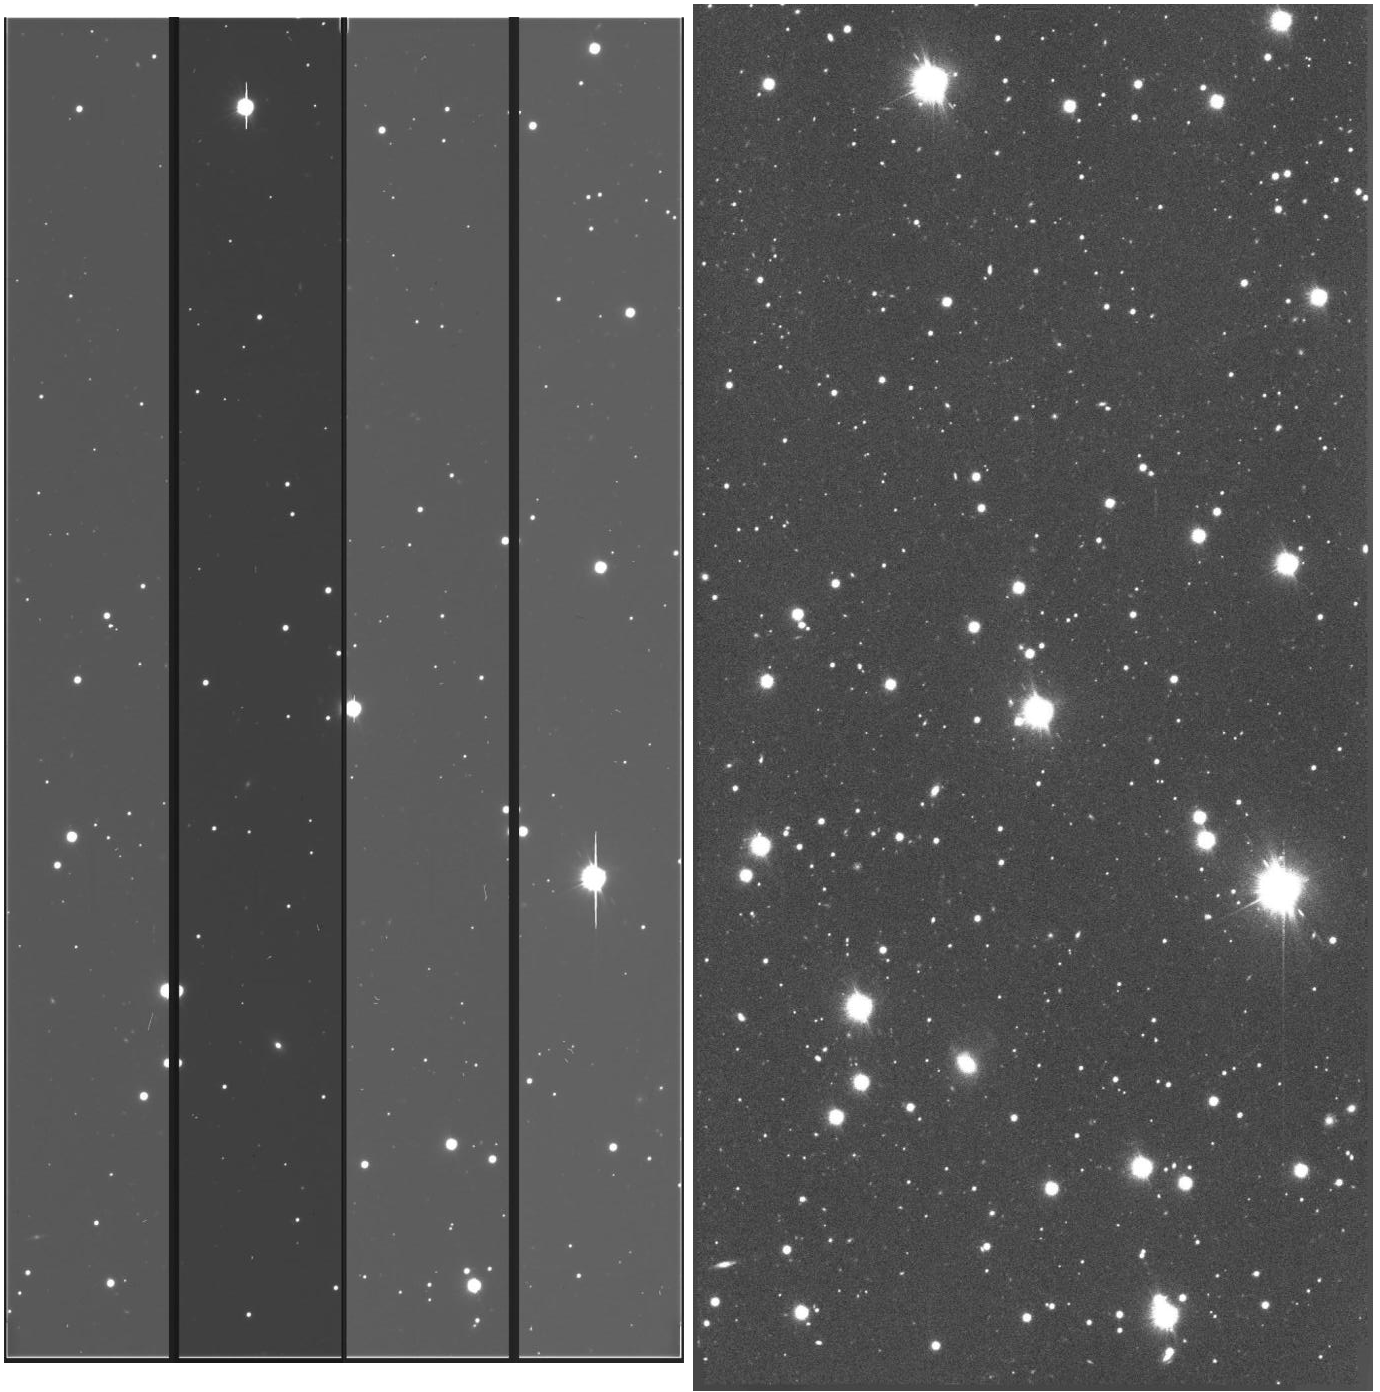
\includegraphics[angle=-90,width=0.8\columnwidth]{figures/raw2calexp.png}
\caption{Raw image (top) and the calibrated exposure (bottom).}
\label{fig:raw2calexp}
\end{figure}

On face value, enabling reprocessing of LSST data using the LSST data reduction pipelines, would at least guarantee repeatability and reproducibility. But by design the LSST data reduction pipelines can, and already do, support many different instruments, such as most major instruments that are currently in use: Dark Energy Camera (DECam), Hyper-Suprime Cam (HSC), SDSS and Canada-France-Hawaii Telescope (CFHT).

Exposing the Science Pipelines functionality through a common interface would pave the way towards standardization of data reduction pipelines, allow access to state of the art astronomical data processing algorithms as well as allow the definition and execution of completely new custom written pipelines, since by design Science Pipelines allow algorithms to be supplemented, replaced or implemented anew. 

Focusing on cloud computing allows us to scale not only the compute resources required but their pay-as-you-go philosophy allows for cost optimization. The global nature of the cloud also facilitates faster and easier data sharing and data access between different scientific communities. 


%%%%%%%%%%%%%%%%%%%%%%%%%%%%%%%%%%%%%%%%%%%%%%%%%%%%%%%%%%%%%%%%%%%%%%%%%%%%%%%%
\section{Technology Stack}
\label{sec:techstack}

While cloud technology was adopted very quickly by some scientific communities and the IT industry, it's adoption by the Astronomical community was slow. Much of the legacy code is designed with the assumption that the data exists locally, or in general that there exists a globally accessible file system, that the processing is some form of batch processing and are in general not state agnostic systems. While it is possible to create similar systems in the cloud, the cloud infrastructure is generally not conducive to such design and is more oriented towards shared-nothing filesystems, containerization and near-data processing architectures. 

To achieve our goals we have to resort to new additions to the legacy codes and tools and to add functionality where it is missing. These tools and code changes are described in mode details in sections \ref{subsec:scipipe} and \ref{subsec:pegasuscondor}, while section \ref{subsec:aws} describes the used cloud services

As aforementioned, astronomical data reduction pipeline consists of many individual steps. Steps, generally speaking, need to be ordered as subsequent ones depend on data products of previous one and each step can require significantly different resources than the previous steps. To achieve scalability, while maintaining required resource allocation flexibility, we use a workflow manager, to which we describe and submit a workflow, and a resource manager, through which we procure required resources. The workflow description is provided by the LSST Science Pipelines and consists of individual jobs targeting single datasets, the description of each jobs required resources as well as the interdependence of different jobs in the workflow. 
\begin{figure}[htb]
\centering
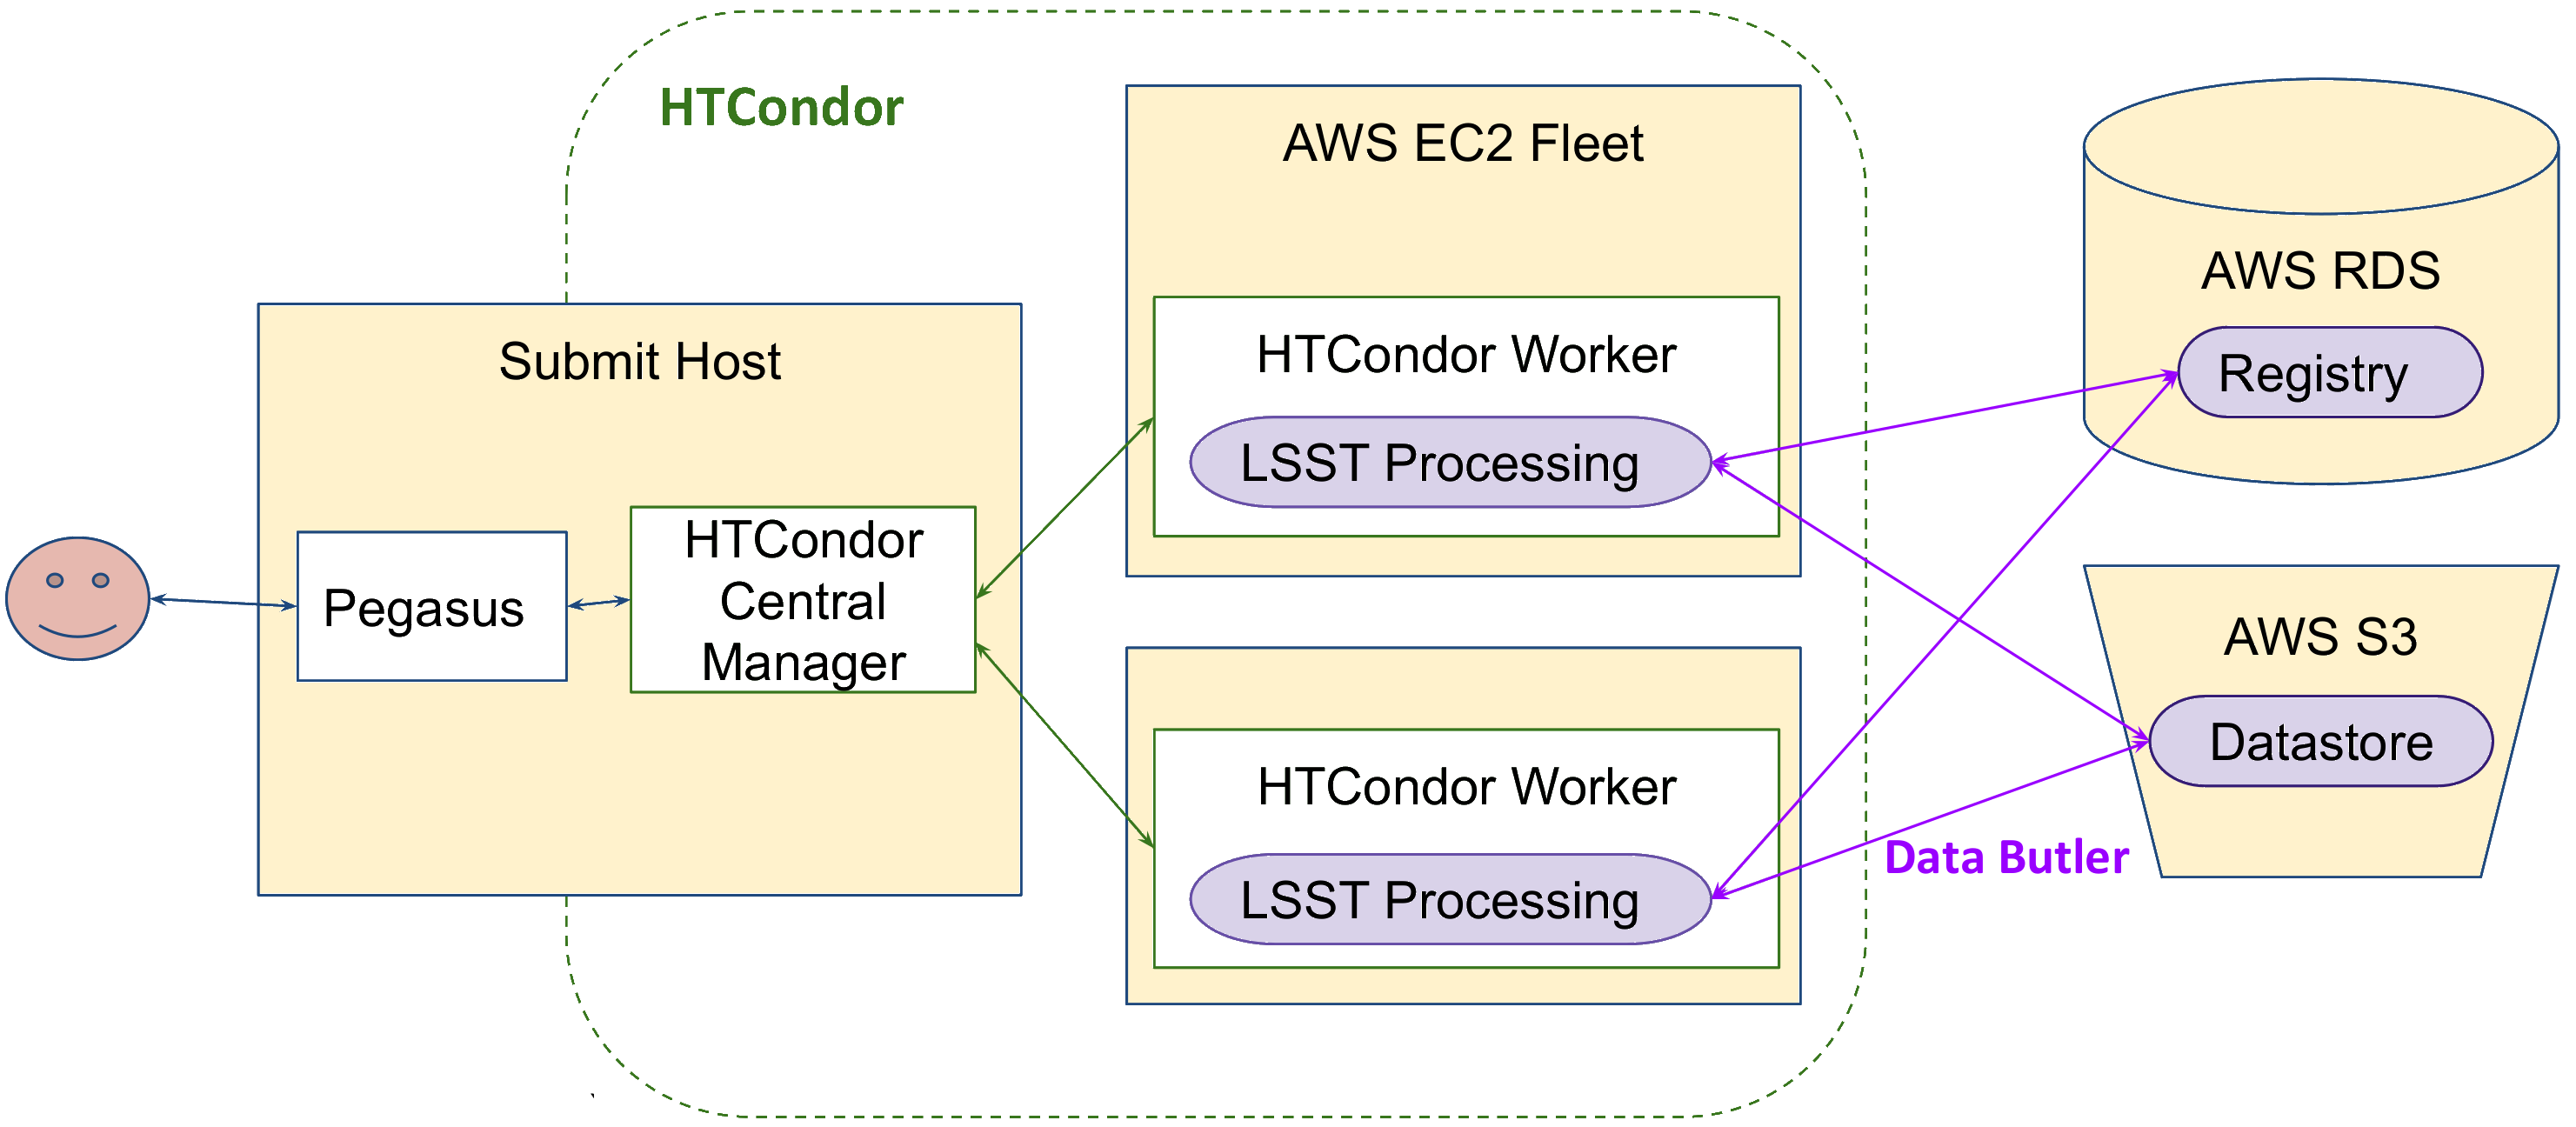
\includegraphics[width=\columnwidth]{figures/workflow.png}
\caption{Diagram of the Technology stack showing its components.}
\label{fig:techstack}
\end{figure}
Scaling is achieved by scheduling as many parallel jobs of the same type as resources allow. When the compute cluster is under-subscribed, such as when the resource requirements are very high or when there are not enough same-type jobs to schedule simultaneously, resource manager will deallocate the idle resources for cost optimization. New resources can also be allocated and dynamically added to the cluster when resource requirements of the jobs change. 

These actions are undertaken from a persistent "master" node where we envision users would, eventually, interact with the components of our system through a Jupyter Notebook like interface. While it is possible to do so currently, the integration of the various used tools and packages with Jupyter is still in its infancy and most of the interaction with the cluster is performed through a terminal via ssh connection.



\subsection{Science Pipelines and Middleware}
\label{subsec:scipipe}

Science pipelines represent state of the art in astronomical data reduction. They consist of variety of configurable Tasks that can be chained into a pipeline. Such pipeline is described by a directed acyclic graph (DAG) called a QuantumGraph. Quantum Graph consists of quanta, which is a task applied to a singular dataset. Science Pipelines enable processing of optical and near-infrared astronomical data from a single visit (instrument signature removal, characterization, calibration, coaddition, forced photometry etc) to overarching tasks such as joint calibration that constrains astrometric and photometric measurements across multiple different visits. 

Tasks themselves are agnostic to the used file formats and locations of the data. The input-output (IO) and provenance is tracked through a middleware component called the Data Butler. The main purpose of the Data Butler is to isolate the end user from file organization, filetypes and related file access mechanisms by exposing datasets as, mostly, Python objects. Datasets are referred to by their unique IDs, or a set of identifying references. Data Butler uses an Registry to resolve the dataset references and resolves the location, file format and the Python object/type the files stored in a Datastore are to be read as.

The Registry is almost always backed by an SQL database and the Datastore is usually backed by a shared filesystem. Significant amount of work in this paper was the implementation of a Registry and a Datastore capable of utilizing AWS resources and is described in detail in \cite{dmtn114} and \cite{dmtn137}.

\subsection{Pegasus WMS and HTCondor}
\label{subsec:pegasuscondor}

\href{https://research.cs.wisc.edu/htcondor}{HTCondor} \cite{Thain:2005:HTCondor} provides distributed job parallelization and is a powerful batch system for high throughput computing (HTC). A HTCondor pool is a collection of compute resources, and HTCondor matches job requests with available resources following their job requirements. HTCondor Annex allows HTCondor deployment on cloud resources via acquisition of cloud compute resources external to an existing HTCondor pool. A pool can have multiple annexes, and each annex manages its own lifecycle. Unused compute resources are automatically deallocated after a user-set time spent idling. 

\href{https://pegasus.isi.edu/}{Pegasus} \cite{Deelman:2015:Pegasus} is a workflow management system built on top of HTCondor.
It provides command line and API interfaces for scientists to write an abstract workflow independent of the underlying computing infrastructure. Pegasus workflows are expressed as DAGs and Quantum Graphs are interpretable by Pegasus. Pegasus comes with various tools for data management, f.e. log transfers, and supports different execution strategies by grouping jobs within or across nodes of a DAG.


\subsection{Amazon Web Services}
\label{subsec:aws}

Datastore implements \href{https://aws.amazon.com/s3/}{Simple Storage Service (S3)} as a backend. S3 is an object storage that allows massive amounts of unstructured data, where each object typically is identified by a globally unique identifier, to be stored and accessed in a durable and highly scalable way.

\href{https://aws.amazon.com/rds/}{Relational Database Service (RDS)} is the AWS cloud service that launches and configures databases with ease. PostgreSQL was chosen as the DBMS backend for the Registry. Primary drivers behind PostgreSQL were the ease of deploying in RDS, the common use of PostgreSQL as a Virtual Observatory (VO) Table Access Protocol (TAP) backend, no additional licensing fees usually associated with proprietary software and PostgreSQL's off-the-shelf support for spatial primitives needed for astronomy. The RDS databases can be backed up into snapshots as well as exported to downloadable files on S3.

Elastic Compute Cloud (EC2) is used to acquire compute resources.  EC2 service uses virtualization technology to deliver a variety of different pre-configured instance types optimized for different use cases. Within each instance type there are several different instance sizes comprised of varying combinations of CPU, memory, storage, and networking capacity. Amazon Machine Image (AMI) provides the information required to launch an instance and we provide pre-built CentOS AMIs that contain and configure the required parts of the technology stack fo both master and the workers. EC2 differentiates between "on-demand" and "spot" instances. On demand instances are allocated to users until they are de-allocated by the user, while spot instances are allocated to the user but can de-allocated at any time with a 2 minute warning. Spot instances prices change based on the demand but are on average much cheaper than on-demand instances.

%%%%%%%%%%%%%%%%%%%%%%%%%%%%%%%%%%%%%%%%%%%%%%%%%%%%%%%%%%%%%%%%%%%%%%%%%%%%%%%%
\section{Example Workflow}

The example workflow is based off of the well understood, well characterized HSC Release Candidate dataset\footnote{\url{https://jira.lsstcorp.org/browse/DM-11345}} tract 9516. This dataset is reprocessed using Rubin Obs. compute resources every two weeks in order to characterize the scientific validity and performance of the algorithms as they are being developed. The workflow consists of initialization, instrument signature removal, characterization and calibration jobs. Initialization job is responsible for correctly setting up metadata in the Registry. There are 6787 instrument signature removal (ISR) jobs. ISR removes image features that are the results of instrument flaws. Characterization consists of modeling the background, point spread function (PSF), repairing cosmic ray traces, detecting and measuring bright sources and measuring aperture correction. There are, again, 6787 characterize tasks in the workflow. Finally the calibration tasks, using PSF and aperture correction from previous step, detect all sources on the image and perform astrometry and photometry on the image. The workflow is shown on figure \ref{fig:demo-workflow}.
\begin{figure}[htb]
\centering
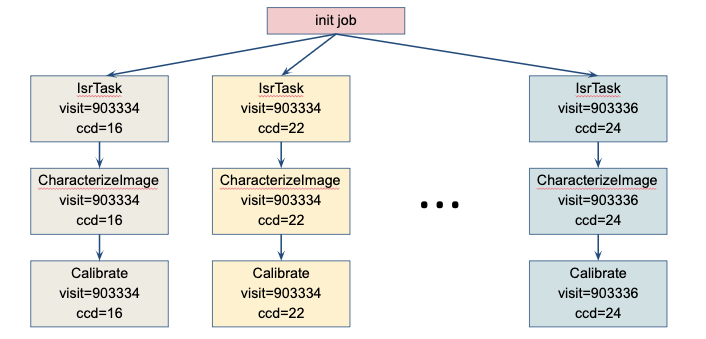
\includegraphics[width=\columnwidth]{figures/demo-workflow.png}
\caption{Example workflow on which performance and scalability was tested.}
\label{fig:demo-workflow}
\end{figure}
The total size of the input data is 0.2TB and the size of output data is approximately 2.7TB. In number of visits processed this represents approximately 11\% of the number or expected Vera Rubin telescope visits. Because each LSST image will be approximately twice the size of a single HSC image, in terms of data volume the example workflow represents approximately 2\% of a night. The scaling between processed data volume and number of visits is a function of observed part of the sky, regions with many objects will on average take longer to process, and the scheduling overheads which themselves are a function of clustering and other execution optimization parameters. Figure \ref{fig:raw2calexp.png} shows the comparison between the raw input image and the output data, a calibrated exposure.


\section{Performance, scalability and cost}

Example workflow was tested against multiple different instance types and instance sizes. The tests were performed on on-demand and on spot instance types. The wall time is the cumulative value of execution times of all Tasks in the Quantum Graph, the scheduling and execution overhead. Results are summarized in table \ref{tbl:cost}.  

The initialization job takes on average 22-30 minutes. This time should not be considered when scaling the execution times to larger datasets because the initialization job is required to run only once per each new output collection and thus would not be run again for any subsequent processing steps or would it be run multiple times if the DAG contained more Tasks. 

Pegasus and HTCondor offer comprehensive and very detailed control over scheduling and execution of jobs. However, as discussed in section \ref{sec:techstack}, these tools were designed and optimized primarily with a more classical HPC computing architectures in mind and the adopted default values for many parameters that control every aspect of execution reflect that. In the initial naive implementation we have encountered various issues in stage-in and out phases of the workflow execution. Namely Quantum Graph nodes, i.e. Quanta, are pickle files. There is about a total of nearly 6GB of these files. Because much of this new functionality are effectively wrappers around legacy code, the default stage-in part of the workflow was performed by uploading the pickle files from master to all the workers. Or, as another example, all log files would all be transferred in stage-out phase of the workflow  from the workers directly to the master. This presents a very large IO bottleneck since without a shared file-system these jobs, in the background, rely on ftp, sftp, rsync and other internet transfer protocols. 

Additionally, the default parameters assumed by various cloud services themselves would presented various different bottlenecks. PostgreSQL Registry, for example, was a new Registry written for Middleware component with this specific application in mind. Science Pipelines were never tested with PostgreSQL as the Registry's DBMS backend. Quickly it became apparent that the various ways views were used in the Middleware's DB schema, were not optimal for execution on PostgreSQL. Similar issues were discovered with the default values of PostgreSQL server parameters, such as maximal allowed number of connections, cache size per connection etc., and IO limitations of EBS drives, often hidden from plain sight by burst credits,  that were mounted on the instances themselves. 

After initial testing it quickly became apparent that these issues lead to poor performance, marked in table \ref{tbl:cost} with light gray background. Resolving many of these issues, moving Pegasus staging into S3, better job clustering, better indexing schemes, materialized views, larger cache values and more appropriately scaled EBS drives achieved performance increase and a cost decrease of 40 to 60 percent. The most jarring comparison of the performance of the implementation were run 20200130T021620, which took 4 hours and 14 minutes and cost nearly 70\$ and run 20200228T014417 which took 1 hour and 54 minutes and cost just shy of 26\$. When the same workflow was executed on spot instances, instead of on-demand instances, the total cost was an entirety of 6.24\$. Instance size and type of the workers on which the three workflows were executed were the compute optimized c5.2xlarge instances, each of which had 8 vCPUs, 16GB of RAM and up to 10Gbps of bandwidth. The actual CPUs on the instances were either the 1st or 2nd generation Intel Xeon Platinum 8000 series processor (Skylake-SP or Cascade Lake) with a sustained all core Turbo CPU clock speed of up to 3.6 GHz. Each job requested a single vCPU. 
\begin{table*}[t]
\centering
    \begin{tabular}{c c c c c c }
    Run name  & Instance count & Cost & Wall Time & Comment \\
    \hline \\
    \multicolumn{5}{c}{m5.xlarge} \\
    \hline \\
    \rowcolor{lightgray}
    20200116T213148  & 25  & 24.34  & 5h39m & - \\
    \rowcolor{lightgray}                        
    20200115T172359  & 50  & 42.15  & 3h50m & - \\
    \rowcolor{lightgray}                        
    20200116T175704  & 100 & 42.97  & 3h18m & - \\
    20200309T135739  & 25  & 24.72  & 5h35m & - \\
    20200309T194101  & 50  & 25.76  & 3h8m  & - \\
    20200309T225436  & 100 & 19.40  & 2h39m & Compute resources not allocated for 32m43s after scheduling the jobs.\\
    \hline \\                                                 
    \multicolumn{5}{c}{c5.2xlarge} \\
    \hline \\
    \rowcolor{lightgray}                                        
    20200127T010224  & 25  & 27.33  & 3h8m  & - \\
    \rowcolor{lightgray}                         
    20200127T162240  & 50  & 50.45  & 3h16m & - \\
    \rowcolor{lightgray}                         
    20200128T192127  & 50  & 67.48  & 3h38m & - \\
    \rowcolor{lightgray}                         
    20200128T234142  & 50  & 54.62  & 3h58m & - \\
    \rowcolor{lightgray}                         
    20200129T034251  & 50  & 68.59  & 4h14m & - \\
    \rowcolor{lightgray}                         
    20200129T184318  & 50  & 51.34  & 3h22m & Replenished burst balance. \\
    \rowcolor{lightgray}                         
    20200129T221952  & 50  & 58.47  & 3h24m & Replenished burst balance.  \\
    \rowcolor{lightgray}                        
    20200130T021620  & 50  & 69.28  & 4h14m &  -  \\
    20200302T222936  & 25  & 26.19  & 4h2m  & Wall time is wrong, job forgotten. \\
    20200227T232007  & 50  & 26.72  & 1h54m & - \\
    20200228T014417  & 50  & 25.78  & 1h48m & Optimal cluster size. \\
    20200302T180554  & 100 & 47.08  & 1h48m & Under-subscribed cluster. \\
    20200302T210301  & 100 & 32.72  & 1h18m & A more appropriate cluster size than 180553 but still not optimal. \\
    \hline \\                
    \multicolumn{5}{c}{c5.xlarge} \\                                
    \hline \\
    \rowcolor{lightgray}                               
    20200123T165014  & 25  & 23.22  & 6h18m & Annex did not de-allocate automatically accidentally restarted the master node. \\
    \rowcolor{lightgray}                      
    20200126T175516  & 50  & 25.81  & 6h7m  & - \\
    \rowcolor{lightgray}                      
    20200123T232152  & 100 & 44.86  & 3h11m & - \\
    20200305T182023  & 25  & 23.38  & 5h45m & Potentially overestimated pricing. \\ 
    20200305T182023  & 50  & 27.43  & 3h41m & Forgotten run timings and cost are overestimated. \\
    20200306T062555  & 100 & 27.36  & 2h2m  & - \\
    \hline \\
    \multicolumn{5}{c}{Spot} \\                                     
    \hline \\
    20200310T191539  & 200 & 28.21 & 1h58m & Instance type and size: m5.large \\
    20200310T183810  & 50   & 6.24  & 1h59m & Instance type and size: c5.2xlarge
\end{tabular}
\caption{Caption}
\label{tbl:cost}
\end{table*}






%\begin{table*}[t]
%\centering
%    \begin{tabular}{c c c c c c }
%    Run name  & Instance count & Cost & Wall Time & Comment \\
%    \hline \\
%    \multicolumn{5}{c}{m5.xlarge} \\
%    \hline \\
%    \rowcolor{lightgray}
%    20200116T213148  & 25  & 24.34  & 5h39m & - \\
%    \rowcolor{lightgray}                        
%    20200115T172359  & 50  & 42.15  & 3h50m & - \\
%    \rowcolor{lightgray}                        
%    20200116T175704  & 100 & 42.97  & 3h18m & - \\
%    20200309T135739  & 25  & 24.72  & 5h35m & - \\
%    20200309T194101  & 50  & 25.76  & 3h8m  & - \\
%    20200309T225436  & 100 & 19.40  & 2h39m & \specialcell{Compute resources not allocated for \\ 32m43s %after scheduling the jobs.}\\
%    \hline \\                                                 
%    \multicolumn{5}{c}{c5.2xlarge} \\
%    \hline \\
%    \rowcolor{lightgray}                                        
%    20200127T010224  & 25  & 27.33  & 3h8m  & - \\
%    \rowcolor{lightgray}                         
%    20200127T162240  & 50  & 50.45  & 3h16m & - \\
%    \rowcolor{lightgray}                         
%    20200128T192127  & 50  & 67.48  & 3h38m & - \\
%    \rowcolor{lightgray}                         
%    20200128T234142  & 50  & 54.62  & 3h58m & - \\
%    \rowcolor{lightgray}                         
%    20200129T034251  & 50  & 68.59  & 4h14m & - \\
%    \rowcolor{lightgray}                         
%    20200129T184318  & 50  & 51.34  & 3h22m & Replenished burst balance. \\
%    \rowcolor{lightgray}                         
%    20200129T221952  & 50  & 58.47  & 3h24m & Replenished burst balance.  \\
%    \rowcolor{lightgray}                        
%    20200130T021620  & 50  & 69.28  & 4h14m &  -  \\
%    20200302T222936  & 25  & 26.19  & 4h2m  & Wall time is wrong, job forgotten. \\
%    20200227T232007  & 50  & 26.72  & 1h54m & - \\
%    20200228T014417  & 50  & 25.78  & 1h48m & Optimal cluster size. \\
%    20200302T180554  & 100 & 47.08  & 1h48m & Under-subscribed cluster. \\
%    20200302T210301  & 100 & 32.72  & 1h18m & \specialcell{A more appropriate cluster size than 180553 \\ %but still not optimal.} \\
%    \hline \\                
%    \multicolumn{5}{c}{c5.xlarge} \\                                
%    \hline \\
%    \rowcolor{lightgray}                               
%    20200123T165014  & 25  & 23.22  & 6h18m & \specialcell{Annex did not de-allocate automatically \\ %accidentally restarted the master node.} \\
%    \rowcolor{lightgray}                      
%    20200126T175516  & 50  & 25.81  & 6h7m  & - \\
%    \rowcolor{lightgray}                      
%    20200123T232152  & 100 & 44.86  & 3h11m & - \\
%    20200305T182023  & 25  & 23.38  & 5h45m & Potentially overestimated pricing. \\ 
%    20200305T182023  & 50  & 27.43  & 3h41m & \specialcell{Forgotten run timings and cost \\ are %overestimated.} \\
%    20200306T062555  & 100 & 27.36  & 2h2m  & - \\
%    \hline \\
%    \multicolumn{5}{c}{Spot} \\                                     
%    \hline \\
%    20200310T191539  & 200 & 28.21 & 1h58m & Instance type and size: m5.large \\
%    20200310T183810  & 50   & 6.24  & 1h59m & Instance type and size: c5.2xlarge
%\end{tabular}
%\caption{Caption}
%\label{tbl:cost}
%\end{table*}





%\begin{table*}[t]
%\centering
%\begin{tabular}{c|c|c|c|c|c|c }
%Run name & Type and size & Instance count & Cost & Wall Time & Spot & Comment \\
%\hline 
%20200302T222936  & c5.2xlarge    & 25   & 26.19  & 4h2m   & No & Wall time is wrong. \\
%20200227T232007  & c5.2xlarge    & 50   & 26.72  & 1h54m  & No & - \\
%20200228T014417  & c5.2xlarge    & 50   & 25.78  & 1h48m  & No & Optimal cluster size. \\
%20200302T180554  & c5.2xlarge    & 100  & 47.08  & 1h48m  & No & Under-subscribed cluster. \\
%20200302T210301  & c5.2xlarge    & 100  & 32.72  & 1h18m  & No & \specialcell{Better than 10301, but still \\ not optimal cluster size} \\
%20200305T182023  & c5.xlarge     & 25   & 23.38  & 5h45m  & No & Overestimated pricing. \\ 
%20200305T182023  & c5.xlarge     & 50   & 27.43  & 3h41m  & No & Timings and cost slightly off. \\
%20200306T062555  & c5.xlarge     & 100  & 27.36  & 2h2m   & No & - \\
%20200309T135739  & m5.xlarge     & 25   & 24.72  & 5h35m  & No & - \\
%20200309T194101  & m5.xlarge     & 50   & 25.76  & 3h8m   & No & - \\
%20200309T225436  & m5.xlarge     & 100  & 19.40  & 2h39m  & No & \specialcell{Compute resources %accidentally not allocated for \\ 32m43s after the jobs got scheduled.}\\
%20200310T191539  & m5.large      & 200  & 28.21 & 1h58m   & Yes & - \\
%20200310T183810  & c5.2xlarge    & 50   & 6.24  & 1h59m   & Yes & - \\
%\end{tabular}
%\label{tbl:cost}
%\end{table*}

%%%%%%%%%%%%%%%%%%%%%%%%%%%%%%%%%%%%%%%%%%%%%%%%%%%%%%%%%%%%%%%%%%%%%%%%%%%%%%%%
\section{Discussion}

We identify two major obstacles to adoption of such a system: difficulty of use, including both the significant amount of initial familiarization with novelty cloud services and perceived dificult-ness {\color{red} andy please help with this sentence} of running and managing the workflow and resources. 

Costing estimates were performed for a more encompassing workflow than the example workflow, it additionally included coaddition and coaddition source measurements, with the same dataset in \cite{dmtn137}. Naive runs of the workflow on AWS cost approximately 95\$ but the workflow cost is dominated by the various bottlenecks we identified in the example workflow as the larger workflow is not yet optimized in the same manner as the example workflow. In \cite{dmtn135} cost estimates were performed for the larger workflow executed on existing Rubin Observatory compute resources predicting a cost of 36\$ for the workflow. Given that the further efforts in characterizing the workflow resource requirements and subsequent optimizations produce similar cost wall time reductions and cost decrease the cost for running the workflow on AWS would be in a much more comparative 38\$ to 57\$ range. Many changes were already made and incorporated into the code that mitigate many of the mentioned bottlenecks. 

Our performance and cost scaling tests indicate that the wall time of a workflow scales linearly with the number of vCPUs used. Therefore a test with 200 m5.large (400 vCPUs) instances finishes in the same walltime as a 50 c5.2xlarge instances (400 vCPUs). This seems to match the performance observed by Rubin Obs test runs. The cost however varies drastically, however. Optimizing costs for a general Quantum Graph is very challenging because the cost is mainly the function of wall-clock offset by the approximately constant cost of the RDS instance and monotonically growing S3 storage. The wall-clock however is a function of instance type and instance size, which is in turn constrained by the task resource requirements. It is crucial the have a very good characterization of each individual task requirements to be able to allocate resources in the most optimal manner. This however is hindered by the fact that resource allocation is not yet easily handled in a dynamical manner where users could adopt a submit-and-forget style of data processing. Adding more fine grained control, possibly defined in the Quantum Graph itself, that would allow for launching or targeting job execution to particular resources tailored specifically to that type of job would be a great improvement to the current workflow and resource management system in this context.

In general the scaling performance does not seem to be limited by IO or connection bandwidth on the workers mainly due to the distributive properties of S3 for typical file sizes in the Science Pipelines. The upper limit is generally set by the size of the instance that hosts the Registry. While scaling out to many workers seems to work, since all jobs need to contact the registry, there is an actual upper limit to the number of workers one might execute on simultaneously. This limit is set by the maximum number of simultaneous connections, and maximum allowed number of locks per connection, that are in turn dependant on the available cache size of the RDS instance. The largest RDS instance available is the db.m5.24xlarge with 96 vCPUs, 384GB of memory and 14000 Mbps of write speed to the attached EBS drives but the associated costs of such on-demand setup soon become prohibitive, with estimated monthly cost of nearly 12500\$. 

In a setup where this functionality is offered as a service, however, it is possible to significantly amortize these costs by procuring reserved instances instead. In that case it is possible to achieve 40\% discount by reserving such an instance for a year, 60\% for three years and it is also possible to negotiate pricing for longer reservation times with AWS directly. Similar savings can be achieved for master, or indeed any other persistent, instances as well. 

%%%%%%%%%%%%%%%%%%%%%%%%%%%%%%%%%%%%%%%%%%%%%%%%%%%%%%%%%%%%%%%%%%%%%%%%%%%%%%%%
\section{Conclusions}

We motivate a use case for a gateway to astronomical data science processing in the cloud based on the ever growing data volumes produced by new astronomical sky surveys and the standardization of astronomical image processing. We propose a design for the backend to one such gateway based on the LSST Science Pipelines by utilizing Pegasus WMS as a workflow manager and HTCondor, and condor\_annex, as the resource manager. We demonstrated that performance and costing are not significantly impacted by the transition to the cloud. We also stress the importance of well characterized workflows and the impact that has on both performance and costing. We describe how it is possible to optimize sets of similar tasks in the workflow and identify missing functionality that would enable easier use of the proposed gateway. We additionally identify and briefly discuss, Jupyter Notebook a potential front-end interface choices given it's wide adoption within Astronomy. 



%%%%%%%%%%%%%%%%%%%%%%%%%%%%%%%%%%%%%%%%%%%%%%%%%%%%%%%%%%%%%%%%%%%%%%%%%%%%%%%%

\bibliographystyle{ieeetr}
\bibliography{bibliography}
\section{Acknowledgements}
\noindent We would like to that Rubin Observatory and the AWS PoC group which were instrumental in testing and eventually adopting and committing to maintaining much of the code written that was required to facilitate AWS processing. 
\clearpage
\end{document}
